\chapter{Methodology}
\label{chap:meth}
\begin{markdown}

This chapter presents the methodology used when developing the PTX.jl
library. Alternative approaches are introduced and discussed with
reasoning for the choices made. Section \ref{sec:meth:ptx} gives a
overview of the library.

# Julia subset for Kernel definition #

For the PTX.jl library, a strict subset of the Julia language features
is defined. The selection of the features was guided by simplicity
of implementation and relevance in GPU applications.

## Kernel language ##
\label{sec:meth:kernel}

The kernel language consists of a few key data types and simple control
structures. The kernel function can call any number of functions, as
long as all functions in its call graph is inlined back into the
kernel function. This can be ensured with the _@inline_ macro. Inside
the kernel, the OpenCL built-in functions described in Section
\ref{sec:meth:built-ins} are available.

### Data types ###

The kernel languages primitive types are listed in Figure \ref{tab:datatypes}.

\begin{figure}[H]
  \centering
  \begin{tabular}{|l|}
  \hline
  Int32\\
  Int64\\
  Float32\\
  Float64\\
  \hline
  \end{tabular}
  \caption{Data types of the Kernel language}
  \label{tab:datatypes}
\end{figure}

In addition to the four primitive types, the language contains a fixed
size vector type, _GPUArray_. This type is implemented partly in Julia
and partly in OpenCL C. The translation of the type is defined in
Section \ref{sec:meth:idea}

### Control Structures ###

A limited set of control structures are provided by the kernel
language. The set is presented in Figure \ref{tab:control}.

\begin{figure}[H]
  \centering
  \begin{tabular}{|l|}
  \hline
  for\\
  if-else\\
  while\\
  \hline
  \end{tabular}
  \caption{Control Structures of the Kernel language}
  \label{tab:control}
\end{figure}

Note that in order to use the _for loop_, the loop must be so short
that it is unrolled.

### Built-in function (OpenCL) ###
\label{sec:meth:built-ins}

The kernels specified in the PTX.jl library have access to a subset of
the built-in function defined in OpenCL \cite{opencl}. The most
important parts of the subset is shown in Figure \ref{fig:meth:built-ins}

\begin{figure}[H]
  \centering
  \begin{tabular}{|l|}
    \hline
    get\_work\_dim\\
    get\_global\_size\\
    get\_global\_id\\
    get\_local\_size\\
    get\_local\_id\\
    get\_num\_groups\\
    get\_group\_id\\
    barrier\\
    \hline
  \end{tabular}
  \caption{Subset of built-in functions}
  \label{fig:meth:built-ins}
\end{figure}

For reference on the functions in \ref{fig:meth:built-ins}, consult the OpenCL Specification.

# Implementing the fixed size vector type #

There are two methods considered to implement the types of the kernel
language. On the one hand, the types can be realized by implementing
the full Julia abstraction on the GPU. On the other hand, one can look
at the implementation or arrays in existing GPU languages as OpenCL C
and CUDA and translate the vector to these. These two choices both
have their benefits and drawbacks explored in the next sections.

## A full Julia implementation ##

Implementing the vector abstraction from Julia, involves including
bounds checking and exception handling. This will give the programmer
a familiar interface to the type and ease development, and as well
improve programmer productivity when writing kernels. With a correct
implementation, the Julia semantics would be continued on the GPU. The
implementation is complicated by the fact that extra data types must
be defined on the GPU and new copy functions must be added. The method
does not trivially imply an efficient implementation, as there will be
overhead both on element access and data movement.

## A low level implementation ##
\label{sec:meth:arrays:low-level}

Implementing the vector type as an unboxed array (the type of
CUDA/OpenCL C), implies getting rid of size information and leaving
the task of bounds checking to the programmer. This approach is the
simpler of the two, as the implementation of an unboxed array is quite
straightforward. On the upside, this will enable integration with
existing tools like the CUDA.jl or OpenCL.jl libraries for transferring
data to and from the GPU, as these expect the data to be unboxed arrays
on the GPU. This method produces efficient code trivially, as there is
no overhead compared to existing low level solutions.

## Choosing the Low level implementation ##

The Low Level implementation is chosen as it is simpler to implement
and will provide efficient code without resolving to custom
optimization. This makes the implementation feasible in the time
window and upholds the focus on a fully working system.

# External library vs. component of the compiler #
\label{sec:meth:lib-b-comp}



An important choice when making software is how to distribute
it. Usually this comes down to; either as a part of a lager system,
or as an external self sufficient component.

### Part of the compiler ###

The obvious placement of a software component that generates code for
a programming language, is in the code generator module of the
_compiler_/_interpreter_. This enables the module to access the AST of
the language in an in-memory format. This also implies that the source
code of the compiler has to be changed for adoption of the component.

### External library ###

An alternative approach is to implement the component as a separate
_library_. In order to do so we need to get the AST in some other
way. This enables the new target to be used without changing the
compiler.

### Other efforts underway ###

The compiler approach is, according to the Julia mailing list
\cite{julia-dev}, in the making. The first draft was so deeply
intertwined with the current code generator, that the authors decided
not to publish their work. A refactoring of this version is underway.

### Choosing the library ###

In light of the concurrent effort, and the fact that the simplistic
design taken in PTX.jl enables a library approach, this approach was
chosen. This enables easy adoption, rapid prototyping and improvements
to the library. Even though PTX.jl is a separate library, the LLVM
optimization passes developed for the library should be easy to
integrate into a future compiler component with a PTX code generator.

# The PTX.jl library #
\label{sec:meth:ptx}
  
The PTX.jl library generates NVIDIA PTX code from a kernel defined in
the Julia programming language. The library is developed as a Julia
module and can easily be included in a Julia program. It inter-opts
with existing CUDA libraries written for Julia. 

## Main idea ##
\label{sec:meth:idea}

The main idea for generating the GPU code, is to substitute Julia
arrays with unboxed arrays, by providing a low level implementation of
the methods operating on the arrays. By disabling inlining for the
functions operating on the array types, the LLVM IR generated
resembles a high level description of the kernel. This description can
be translated into a low level implementation on unboxed arrays. This
fact is exploited, and low level implementation of the high level Julia
functions _getindex_ and _setindex_ are linked with the code. In
addition, to support the OpenCL programming model, built-in functions
like _get_global_id_ is also linked.

\begin{figure}[H]
  \centering
  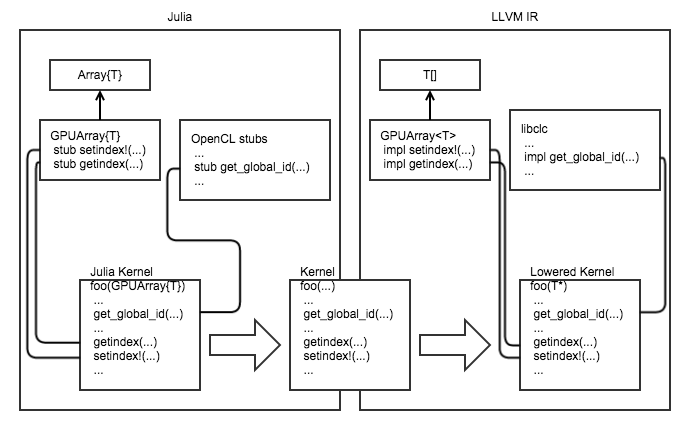
\includegraphics[width=1\textwidth]{body/figures/lowering_schematic.png}
  \caption{Schematic for lowering kernel functions}
  \label{fig:lowering}
\end{figure}

In Figure \ref{fig:lowering}, the kernel is linked to the Julia stubs
for getindex, setindex and get_global_id on the left side. The
parameter type for the function is a Julia boxed array. The function
parameter is replaced by the unboxed version of the array and the type
is propagated through the function. As the GPUArray only
implements\footnote{This is using terminology from OOP. Julia does not
  use this terminology, but the language features does enable OOP. In
  Julia terminology the only functions that have methods that accept
  GPUArray as parameters are setindex and getindex.} the functions
setindex and getindex, we are guarantied that the array is not
referenced in other contexts than through these accessor functions.
Linking these two methods with implementations for unboxed arrays
concludes the lowering of the functions. The remaining task is to
provide implementations for the OpenCL built-in functions. This is done
by linking to an open source library called libclc \cite{libclc}.

  
\end{markdown}
